\section{Introduction}

Complex multicellular organisms exist despite unicellular life growing biomass with substantially greater efficiency \citep{lynch2024bioenergetic}.
Division-of-labor explanations \citep{Saunders1976,corning2015synergistic,niklas2014evolutionary,Bell1997} recoup only part of this metabolic cost, motivating alternate accounts based on neutral ratcheting of near-neutral redundancies \citep{Gould1988,lynch2003origins,muozgmez2021constructive} or niche construction, whereby feedback from organisms reshapes environmental context in ways that favor complex traits \citep{odlingsmee2003niche,taylor2004niche,laland2014niche}.
Though implicated in biological multicellularity \citep{niklas2014evolutionary,boraas1998phagotrophy,yoshida2003rapid}, the causal role of \textit{de novo} niche construction in promoting complexity during early multicell evolution remains experimentally untested \citep{goldsby2012task,bozdag2023denovo,ratcliff2012experimental,kalambokidis2023multispecies}.

\section{Experimental System}

\input{fig/overview.tex}

We test this using DISHTINY \citep{moreno2019toward}, a digital model system in which cell-like programs populate a 2D grid, replicating via asexual budding either to grow an existing multicell group or to found a new one (Figure~\ref{fig:overview}).
Neighboring cells --- within and between groups --- compete for space, share energy, exchange messages, and sense each other's state, creating feedback between evolved phenotypes and environmental context.
Cell behavior arises from tag-based activation of genome subprograms \citep{lalejini2018evolving,moreno2023matchmaker}.
Across 40 replicate evolving populations, we assay genotype complexity (genome sites deleterious when knocked out), phenotype complexity (distinct adaptive cell input/output interactions), morphology, and competitive fitness to test whether niche construction promotes and sustains complexity.

\section{Results}

Among replicates, one lineage sustained genotype and phenotype complexity exceeding $3\times$ IQR of all others, alongside a multi-stage patterned life history: an initial elongated ``cigar-like'' morphology (arising at passage 15) followed by an irregular ``box-like'' secondary growth phase (passage 45).
Tracing this case-study lineage across 100 sequential passages, we identified nine morphologies and repeated abrupt complexity gains coincident with morphological innovation --- e.g., phenotype complexity tripled at the cigar-like transition.

\begin{figure}

\begin{minipage}{\linewidth}
\begin{subfigure}[b]{0.692\linewidth}
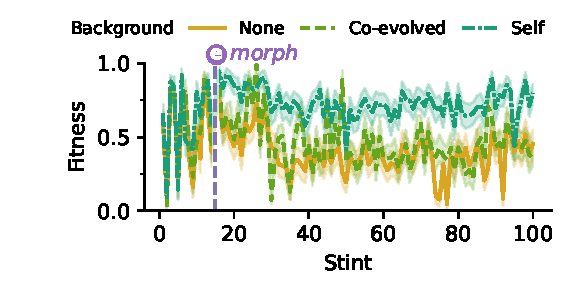
\includegraphics[width=\linewidth, trim=0.8cm 0 0 0, clip]{binder-2025-11-30-external-selfbb-truebb.ipynb/binder/teeplots/2025-11-30-external-selfbb-truebb/hue=kind1+style=kind1+viz=lineplot+x=competition-stint+y=focal-prevalence+ext=.pdf}
\footnotesize
\vspace{-4.25ex}
\caption{stints 0 to 100}
\label{fig:fitness-background:timeseries}
\end{subfigure}%
\begin{subfigure}[b]{0.308\linewidth}
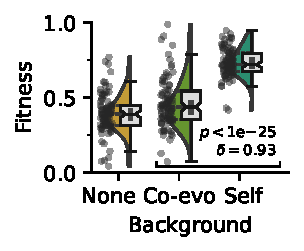
\includegraphics[width=\linewidth, trim=1.3cm 0 0 0.1cm, clip]{binder-2025-11-30-external-selfbb-truebb.ipynb/binder/teeplots/2025-11-30-external-selfbb-truebb/hue=kind+inner=quartile+viz=violinplot+x=kind+y=focal-prevalence+ext=.pdf}
\footnotesize
\vspace{-4.25ex}
\caption{stints 15 to 100}
\label{fig:fitness-background:distribution}
\end{subfigure}
\end{minipage}

\caption{%
\textbf{Patterned growth creates biogenic niche.}
\footnotesize
Around stint 15, fitness of case study strain in self-context diverges significantly above other contexts.
``None'' background competitions are initialized 50\%/50\% between compared strains; otherwise, competitions are initialized 25\%/25\%/50\% between compared strains and background.
Shaded bands are bootstrap 95\% CI.
Mann-Whitney test reported.
}
\label{fig:fitness-background}
\end{figure}


Competing case-study genomes against a cross-replicate ``measuring stick'' panel, we found that fitness in self-context (i.e., against the lineage's own biogenic background) diverged sharply above fitness in co-evolved or background-free context beginning at this cigar-like transition (Mann-Whitney $p<10^{-25}$, Cliff's $\delta=0.93$; Figure~\ref{fig:fitness-background}) --- the lineage's patterned growth constructed a niche favoring itself over other morphologies.

To test whether this niche construction causally sustains complexity, we conducted evolutionary replay experiments: mutagenizing case-study genomes and reseeding populations under either self- or co-evolved biotic context.
Replays retaining self context maintained significantly higher genotype complexity than those with co-evolved context (Mann-Whitney $p<0.01$, $\delta=0.25$) --- an effect that vanished under a higher mutagenic dose, confirming that self-acting biotic selection, rather than generic disruption, locks in complexity.

This pattern generalized across replicates: self-adaptation (fitness advantage in self- versus co-evolved context) correlated positively with both genotype and phenotype complexity (Wald tests, $p=0.01$ and $p=5\times10^{-3}$), rivaling or exceeding correlations attributable to adaptation or drift alone.

\section{Discussion}

These findings show that biotic selection arising from an organism's own niche construction can act as a powerful complexity ratchet, complementing --- and potentially reconciling --- adaptationist and neutralist accounts of complexity evolution.
Because digital multicells reproduce core features of Darwinian evolution while permitting fine-grained causal manipulation \citep{pennock2007models}, this system offers a tractable route to directly test eco-evolutionary feedback hypotheses that are difficult to isolate in biological multicells.
Ongoing work extends these replay and reciprocal-context designs across longer timescales to assess the generality of ecological complexity lock-in.
